\documentclass[12pt,a4paper]{article}
\usepackage{txfonts}
\usepackage{url}
\usepackage[colorlinks, citecolor=blue, urlcolor=blue]{hyperref}
\usepackage[utf8]{inputenc}
\usepackage[spanish]{babel}
\usepackage{amsmath}
\usepackage{amsfonts}
\usepackage{amssymb}
\usepackage{makeidx}
\usepackage{graphicx}
\usepackage{lmodern}
\usepackage{kpfonts}
\usepackage{fourier}
\usepackage[left=2cm,right=2cm,top=2cm,bottom=2cm]{geometry}
\author{Rodriguez Lopez Francisco Javier}
\begin{document}

\begin{center}
\LARGE \textbf{Universidad Politecnica de la Zona Metropoilitana de Guadalajara\\}



\includegraphics[width=7cm]{Upzmg.png} 

\LARGE \textbf{Optoacopladores y Relevadores}\\
\vspace{2cm}
\large \textbf{Nombre: Rodriguez Lopez Francisco Javier.\\
\vspace{0.5cm} Matricula: 18311804.\\
\vspace{0.5cm} Carrera: Ingenieria en Mecatronica.\\
\vspace{0.5cm} Materia: Sistemas Electronicos de Interfaz.\\
\vspace{0.5cm} Curso: septiembre-diciembre del 2019.\\
\vspace{0.5cm} Docente: Moran Garabito Carlos Enrique.}


\vspace{6cm}
\small \textbf{03 de Octubre del 2019}
\end{center}

\section{Introduccion.}
En esta seccion del documento explicaremos todos los apartados del mismo en donde se explicaran todos los paso realizados en la practica realizada con anterioridad.\\
 Primeramente se realizara el objetivo de la practica, omitiendo la explicacion de la introduccion.\\
 En donde se explicara de manera breve el objetivo para realizar esta practica.\\
 En la parte del desarrollo se explicara a detalle el funcionamiento que debe contener el circuito asi como la forma en que se fue realizado ademas de contener el funcionamiento de cada parte del circuito y su explicacion en palabras contextualizadas y simples a partir de este punto se explicara paso a paso cada parte del mismo mencionando cada aspecto de la practica y las previas atenciones que se le debieron de tener.\\
 Aspectos como el armado que se menciono anteriormente sera explicado a detalle asi como los aspectos a cuidar como las caracteristicas que se deben tener por proteccion al mismo circuito y a la placa de control, asi como la programacion correspondiente para el arduino para que  este tenga un correcto funcionamiento y tenga la funcionalidad que se necesita para esta practica en especifico.\\
 Despues de abundar en el procedimiento se mostraran los resultados de la practica, calculos, imagenes y etc, asi como una descripcion para su facil comprension.\\
 Posteriormente se realizaran las correspondientes conlcusiones al respecto de la misma practica y cada uno de los colaboradores  tendra su opinion en este apartado y para finalizar se mostraran las referencias bibliograficas de las fuentes de informacion que se utilizaron en esta.  

 \section{Objetivo:}
Comprender la utilizacion de los integrados en conjunto con los relevadores y los transistores, para establecer un PLC.

\section{Procedimiento:}
En este apartado se realizara la explicacion de la practica.
primeramente se realizaron los caculos de la resistividad del circuito para determinar que valor de resistencias se tendra en uso para las diferentes partes del circuito para evitar la sobrecarga en la placa de control en este caso arduino  estos calculos se basan en los explicados por el docente.\\\\
Teniendo esto en cuenta y siendo realizado de manera correcta se procedera a armar la primera parte del circuito, la primera parte seria tener una fuente de voltaje de 12 v conectada a un push button para despues estar conectada a una resistencia y a un led lo que sera conectado despues a un optoacoplador este optoacoplador tiene la funcion de recibir la señal de la energia (cuestion que regulara o podra ser controlado por el push button y mostrado por el led)\\
Del otro lado del optoacoplador tenemos una fuente de 5v que solo podra ser suministrada a todo el circuito si la primera parte en donde se encuentra el push button esta activada sirviendo como un regulador, la corriente pasara por el optoacoplador y hacia el arduino, no sin antes pasar por una resistencia de alto valor que hace el trabajo de evitar que el arduino se queme ademas de llevar al circuito mientras este apagado al  cero logico para evitar la confusion del mismo debido a los factores ambientales.\\\\
Despues de tener el primer circuito armado o la primera parte la segunda parte de este sera el arduino en donde simplemente se tendra una entrada por donde la parte anterior del circuito pasa y una salida por donde se energiza la otra parte del circuito, en base a esto se realiza la programacion del arduino simplemente con condicionales if y else para esta parte.\\
Al haber concretado dicha seccion teniendo compilado y cargado el programa al arduino se procedera a conectar la primera parte del circuito al mismo.\\\\
Para esta ultima parte de la practica se procedera por armar la parte de la salida del circuito en donde se tendra un led para generar la notificacion de que todo fue realizado con exito, para esta parte los pines de salida (previamente seleccionados en la programacion del arduino) se conectaran hacia un transistor, en este caso el 2n2222 que esta conectado al arduino y a la fuente de 12v que energizara el circuito sera usado un diodo para evitar el retorno de la corriente y asi evitar daños potenciales ya sea a la placa de control o al circuito en si.\\
Al enviar la señal al arduino este la procesara para generar la salida que sera enviada a la segunda parte del circuito en donde el relevador sera activado al igual que el led, estos no seran energizados por completo por el arduino debido a su falta de poder para energizar este circuito por lo que el transistor actuara como una compuerta en donde si en arduino deja pasar la corriente se activara y dejara pasar la corriente proveniente de la fuente externa.\\\\
Nota: en la segunda parte tambien se utilizaron los calculos de las resistencias para el mismo proposito que en la primera seccion.\\\\
Este circuito sera implementado cuatro veces teniendo una configuarcion independiente uno del otro para que asi cada señal sea interpretada  de manera aislada todo se conectara a las mismas fuentes de la misma manera teniendo todo la misma tierra tanto el arduino como todas las partes del circuito.  

\section{Resultados:}
Como ya se explico en el procedimiento, las funciones que cumplen las interfaces tanto de entrada como de salida, y estas siendo controladas por el arduino, que cumple la funcion de control, todos estos juntos hacen la previsualizacion de lo que es un PLC, ya que estos componentes son los mas usadospara la contruccion de estos.\\
Como era de esperarse las funciones que cumplio la interfaz de entrada es ver como este manda señales a traves del voltaje que es llegado a su inicial, en este caso el push botoon, cuando este es presionado, libera su voltaje, haciendo que el control haga su trabajo, que es enviar la señal de entrada al control(Arduino).\\

\begin{figure}[hbtp]
\centering
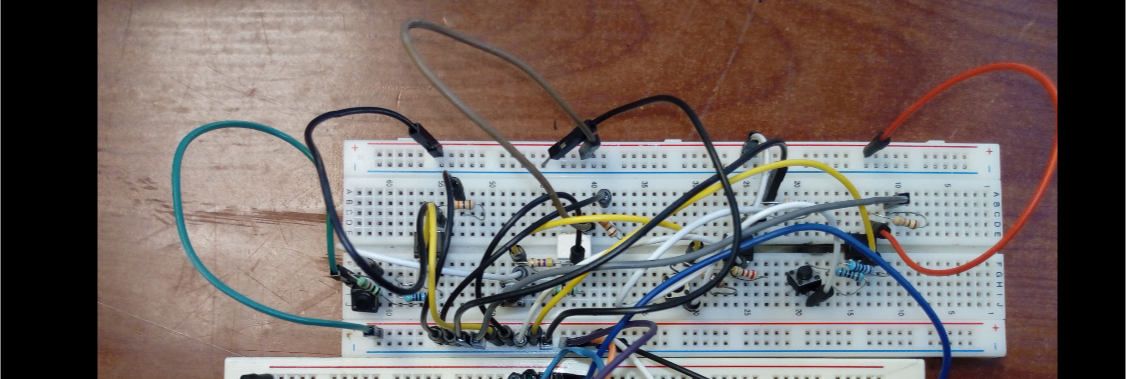
\includegraphics[width=10cm]{Opto.png}
\caption{Interfaz de Entrada}
\end{figure}


En la interfaz de entrada se realizo un calculo el cual nos ayudo a ver el valor de la resistencia que esta conectada en serie con el push botton, este calculo a la par nos deja controlar de mejor manera el voltaje de entrada, para que asi solo lleguen 5V, a el control.
Formula utilizada:
\emph{fourier}
$$ \frac{(V-Vf(IR))}{IF(IR)} $$
En primera estancia, se podria utilizar la Ley de Ohm, pero en este caso, utilizamos otros criterios como el IR, IF y Vf, que son caracteristicas que tiene el integrado que utilizamos(4n25).\\
Obteniendo valores:\\
$$ \frac{(12v-1.5v(150mA))}{60mA(150mA)}= 1308.33 ohm $$
En valor comercial queda como 1220 ohm, en este caso.

Para esto el voltaje pasara a ser de 5v, en donde el control los recibira, para no quemarlo con el voltaje de entrada. todas las tierras estan conectadas entre si, en donde el mismo Arduino, las conecta, ya que todas ellas, van de la par entre los cuatro circuitos que son iguales, tienen que ser dependientes las tierras unas de otras.\\
Para la interfaz de salida, lo que se busca es que los relevadores, es que su NA y NC, se abran esto conseguido despues de que el voltaje recibido, desde la interfaz de entrada, hasta el control, llegue hasta el transistor y este a su vez a la bobina que contiene el relevador, excitando esta y que asi consiga abrir y cerrar, el NA y NC, esto generara el encendido de un Led, que viene en serie con un diodo, y una resistencia.\\
Esto tambien lleva en si un calculo, para la resistencia que esta conectado al Arduino.\\
Formula utilizada:\\
$$ R= \frac{V_{IN}-0.6*HFE}{I_{RELE}} $$
Obteniendo los datos, solo queda ponerlos en la formula.
$$ R= \frac{5v-0.6*200}{50mA}= 1760 Ohm $$
Valor comercial: 2200 ohm.\\
Ya teniendo el valor de esta resistencia, para que ejecute el voltaje necesario, para encender el led, y que el relevador cierre y abra, respondiendo claro al llamado, de la interfaz de entrada. Nos queda conectado como en la imagen.\\

\begin{figure}[hbtp]
\centering
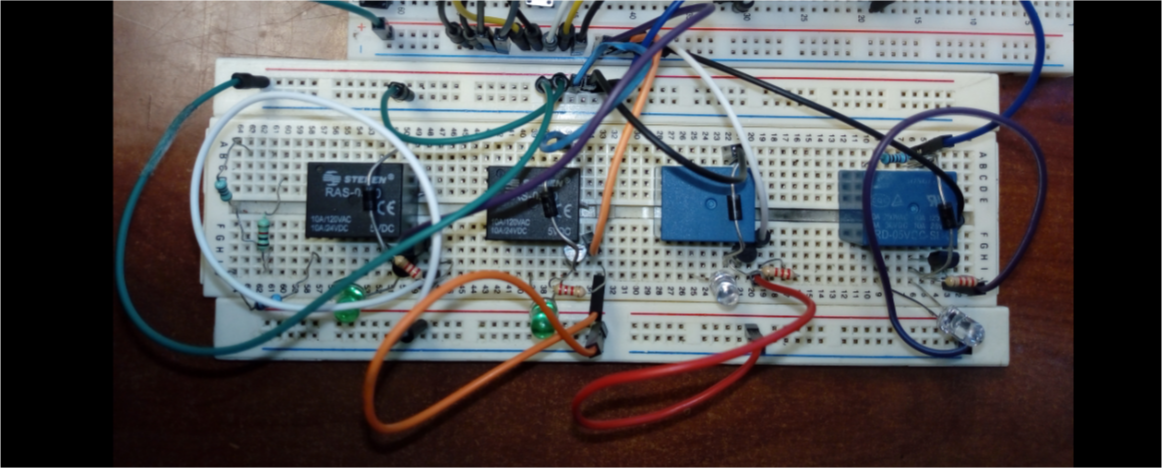
\includegraphics[width=10cm]{Rele.png}
\caption{Interfaz de Salida}
\end{figure}


Ahora si teniendo las funciones, que tomara cada interfaz y el calculo de la misma, el resultado queda como un PLC, en el cual se ejecuta una accion de abierto y cerrado, que en si ejecutan, tanto los relevadores, como los optoacopladores la funcion misma desde el control, guiado por microprocesadores, o chips, en todo caso el Arduino, que nos ayuda a esta valiosa tarea, como la de ejecutar todas las acciones necesarias en esta practica.\\
Visualizacion del circuito en este caso, las interfaces de entrada y de salida.\\

\begin{figure}[hbtp]
\centering
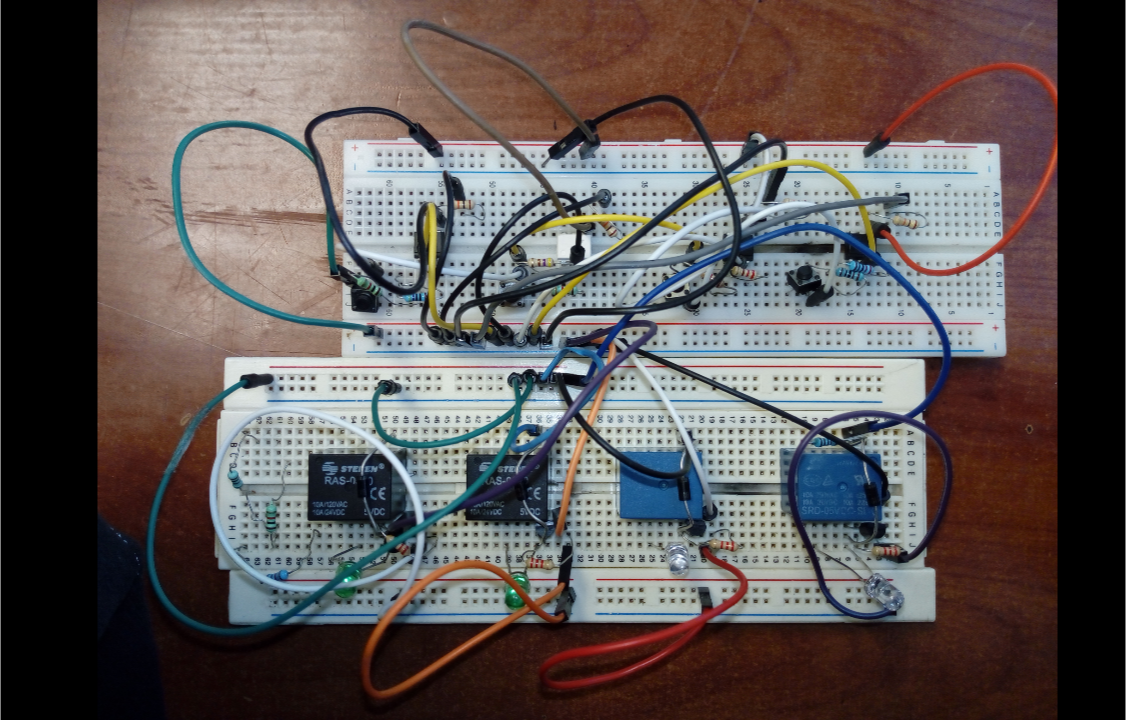
\includegraphics[width=9cm]{Interfaz.png}
\caption{Interfaces en conjunto}
\end{figure}


En esta parte terminamos, siendo este practica de conocimiento industrial, ya que en si, manejamos casi todo desde el control, siendo las interfaces, enviadores de ondas, que en este caso, hacen la accion de ejecucion,el abierto y cerrado del relevador, dada la llegada de la excitacion de la bobina, y el uso del voltaje dado los optoacopladores, y calculos de las resistencias.

\section{Conclusion:}

En terminos generales, la constitucion y acoplamiento de estos materiales, trabajando en conjunto con la llegada de un microoprocesador o chip, hacen el constituyente de un PLC, siendo esto, una generacion de trabajo mas factible y ordenada para cualquier industria, la cual se requiera de un servicio largo,y que impacte varias tareas en conjunto de trabajo pesadas, y de mayor rendimiento, generando todo, desde una terminal.\\
Las ventajas de cada uno de estos componentes, es que todos se acoplan bastante bien a la hora de la realizacion de cualquier trabajo, o accion a ejecutar, en este termino se debe distinguir la labor de cada componente, y sus caracteristicasr ya que si no se tiene bien definido este punto, tu practica puede llegar a ser un cortocircuito generando estragos en tu trabajo.

\section{Referencias Bibliograficas:}
\url{http://www.ieec.uned.es/investigacion/Dipseil/PAC/archivos/Informacion_de_referencia_ISE6_1_1.pdf}
\end{document}